% Patent Application — LaTeX Format
% DETERMINISTIC KNOWLEDGE COMPILATION FROM FORMALLY-STRUCTURED SOURCE ARTIFACTS
% WITH HYBRID STRUCTURAL-SEMANTIC RETRIEVAL AND PROVENANCE-GROUNDED SYNTHESIS

\documentclass[12pt]{article}

\usepackage[T1]{fontenc}
\usepackage[utf8]{inputenc}
\usepackage[margin=1in]{geometry}
\usepackage{setspace}
\usepackage{hyperref}
\usepackage{graphicx}
\usepackage{titlesec}
\usepackage{listings}
\usepackage{xcolor}
\usepackage{enumitem}
\usepackage{cite}
\usepackage{booktabs}
\usepackage{array}
\usepackage{caption}
\usepackage{float}
\usepackage{amsmath}
\usepackage{amssymb}
\usepackage{parskip}

\setstretch{1.2}

% Patent-style section formatting — unnumbered, uppercase
\titleformat{\section}{\normalfont\large\bfseries\centering}{}{0em}{\MakeUppercase}
\titleformat{\subsection}{\normalfont\normalsize\bfseries}{}{0em}{}
\titleformat{\subsubsection}{\normalfont\normalsize\bfseries\itshape}{}{0em}{}

\lstset{
  basicstyle=\ttfamily\small,
  breaklines=true,
  frame=single,
  backgroundcolor=\color{gray!8},
  rulecolor=\color{gray!30},
}

\hypersetup{
  colorlinks=true,
  linkcolor=black,
  citecolor=black,
  urlcolor=blue,
}

\graphicspath{{./}}

% -----------------------------------------------------------------------
\begin{document}
% -----------------------------------------------------------------------

% Patent header — USPTO style
\begin{center}
  {\small U.S. Patent Application}\\[6pt]
  {\LARGE\bfseries DETERMINISTIC KNOWLEDGE COMPILATION\\
  FROM FORMALLY-STRUCTURED SOURCE ARTIFACTS\\
  WITH HYBRID STRUCTURAL-SEMANTIC RETRIEVAL\\
  AND PROVENANCE-GROUNDED SYNTHESIS}\\[12pt]
  {\normalsize Inventor: Eric G.\ Suchanek, PhD\\
  Flux-Frontiers, Liberty Township OH}\\[4pt]
  {\small Application No.\ [PENDING-1] \quad Filed: 2026}
\end{center}

\vspace{1em}\hrule\vspace{1em}

% -----------------------------------------------------------------------
\section*{Cross-Reference to Related Applications}
% -----------------------------------------------------------------------

This application is the foundational patent in a series of three related
applications. U.S.\ Patent Application No.\ [PENDING-2], entitled ``System and
Method for Federated Retrieval-Augmented Generation over Structurally Derived
Heterogeneous Knowledge Graphs,'' and U.S.\ Patent Application No.\
[PENDING-3], entitled ``TreeOfKnowledge: Fractal Forest Visualization of
Compiled Knowledge Graphs with Temporal Animation and Federated Query
Illumination,'' each claim priority to and incorporate by reference the
disclosure of this application. Each of the foregoing applications is
incorporated herein by reference in its entirety.

% -----------------------------------------------------------------------
\section*{Statement Regarding Federally Sponsored Research}
% -----------------------------------------------------------------------

Not Applicable.

% -----------------------------------------------------------------------
\section*{Field of the Invention}
% -----------------------------------------------------------------------

The present invention relates to knowledge representation and information
retrieval, and more particularly to a method and system for compiling
formally-structured source artifacts into structural knowledge graphs using
domain-specific ontologies derived from the formal grammar or schema of each
source domain, and for performing hybrid structural-semantic retrieval over such
compiled knowledge graphs to produce provenance-tagged results enabling grounded,
verifiable language model synthesis.

% -----------------------------------------------------------------------
\section*{Background of the Invention}
% -----------------------------------------------------------------------

Large language models (LLMs) have demonstrated impressive capabilities in
generating coherent text and synthesizing information~\cite{brown2020gpt3,
chowdhery2022palm, touvron2023llama}. However, they suffer from a fundamental
limitation: they are generative systems. When asked a factual question, an LLM
produces an answer by sampling from a learned probability distribution over
tokens conditioned on the prompt. This process does not distinguish between facts
the model has reliably encoded and plausible-sounding sequences it constructs by
pattern interpolation. The resulting phenomenon---commonly called
``hallucination''---is not a failure of implementation but a structural property
of the generative paradigm itself~\cite{ji2023hallucinationsurvey,
maynez2020faithfulness}.

Retrieval-augmented generation (RAG) partially addresses this problem by
providing the LLM with retrieved context before it generates an
answer~\cite{lewis2020rag, guu2020realm}. In standard RAG systems, a query is
encoded into a dense vector and submitted to a vector index that returns
semantically similar document chunks~\cite{johnson2021faiss, karpukhin2020dpr}.
These chunks are prepended to the LLM prompt, and the LLM is instructed to
answer from the provided context.

Standard RAG reduces but does not eliminate hallucination for several reasons.
First, document chunks are semantic units---they capture approximate meaning but
are not formally structured. The retrieval system cannot distinguish a chunk
containing a definitive statement from one containing a qualification, example,
or hypothetical. Second, vector similarity is an approximation: the most relevant
chunks for a query may not be the most semantically similar in the embedding
space~\cite{thakur2021beir}. Third, chunks are not linked by structural
relationships: a function definition chunk has no explicit connection to the
chunks containing functions it calls, imports it depends on, or classes it
implements. The LLM must reconstruct these relationships by generation, creating
an opportunity for hallucination.

The ``needle in a haystack'' problem in retrieval systems refers to the
difficulty of locating a specific, precise piece of information in a large corpus
where that information does not necessarily appear as the most semantically
similar document to the query~\cite{levy2024longcontext}. Standard dense
retrieval ranks by global semantic proximity and has no mechanism to prefer a
structurally adjacent node over a semantically similar but contextually
irrelevant one.

Prior art in knowledge graph construction typically relies on language model
inference to extract entities and relationships from unstructured
text~\cite{pan2024unifyingllmkg, edge2024graphrag, yao2023kgllm}. These
approaches inherit the probabilistic limitations of their extraction models: the
resulting graph contains hypothesized, inferred, or approximated edges that may
not correspond to verified relationships in the source.

What is needed is a retrieval system that is not generative at the knowledge
layer, does not rely on approximate semantic proximity as its sole retrieval
mechanism, and produces results that are structurally exact, provenance-tagged,
and linkable directly to their source. The present invention provides such a
system by applying the methodology of a compiler to the problem of knowledge
graph construction.

% -----------------------------------------------------------------------
\section*{Summary of the Invention}
% -----------------------------------------------------------------------

The present invention provides a knowledge compilation system and method
comprising: a deterministic source parser configured to extract typed nodes and
directed edges from a formally-structured source artifact using an ontology
derived directly from the formal grammar or schema of the source domain, without
language model participation in graph construction; a stable node addressing
scheme encoding the semantic type, source file path, and qualified name or
positional identifier of each extracted entity in a persistent string identifier;
a graph storage layer persisting typed nodes and edges in a relational database;
a semantic indexing layer encoding each node's canonical text representation as a
dense vector~\cite{reimers2019sbert}; a hybrid retrieval engine performing two
sequential stages---a semantic seeding stage that identifies a short ordered list
of entry-point nodes using vector similarity, followed by a structural traversal
stage that expands from those seed nodes through the graph storage layer using
bounded breadth-first search---to produce a ranked list of nodes whose relevance
is determined by structural proximity within the compiled graph rather than by
semantic proximity to the query string alone; a provenance extraction stage that
reads the actual source text at each retrieved node's verified file path and line
span and attaches it to the result record; and a synthesis interface that
presents the provenance-tagged result set to an external language model for
synthesis, ensuring that every fact available to the synthesis model is directly
traceable to a structurally verified source address.

In a preferred embodiment, the ontology used for each source domain is derived
from the formal specification of the domain rather than from human annotation or
machine learning inference. For Python source code, the ontology is derived from
the Python language grammar and abstract syntax tree specification~\cite{python_ast}.
For Markdown and reStructuredText documentation, the ontology is derived from the
CommonMark and RST parse tree specifications. For protein structure data bank
files, the ontology is derived from the PDB file format specification. For legal
statutes, the ontology is derived from the hierarchical structure encoded in the
statute's numbering scheme.

In a preferred embodiment, the compilation process separates into two phases: a
build phase in which the source artifact is parsed, the graph is constructed and
stored, and each node is encoded into a vector and stored in the semantic index;
and a query phase in which no parsing or encoding is performed, queries execute
against the pre-built index and graph, and all results are returned in bounded
time independent of corpus size. This phase separation is analogous to the
separation between compilation and execution in compiled programming language
toolchains~\cite{aho2006compilers}, and confers the same economics: the build
cost is paid once per corpus version; the query cost is paid once per query, at a
fraction of the build cost.

% -----------------------------------------------------------------------
\section*{Brief Description of the Drawings}
% -----------------------------------------------------------------------

\textbf{FIG.~1} is a phase diagram illustrating the separation of the compilation
phase from the query phase, with the build-time operations of parsing, graph
construction, and embedding on the left, and the query-time operations of
semantic seeding, structural traversal, and provenance extraction on the right.

\textbf{FIG.~2} is a data structure diagram illustrating the stable node
addressing scheme, showing how a node identifier encodes the kind prefix, source
file path, and qualified entity name.

\textbf{FIG.~3} is a flow diagram illustrating the two-pass abstract syntax tree
compiler for Python source code, showing the definition extraction pass and the
call-graph and data-flow extraction pass.

\textbf{FIG.~4} is a flow diagram illustrating the hybrid retrieval algorithm,
showing the semantic seeding stage followed by the bounded breadth-first
structural traversal stage, and the composite ranking function applied to the
reached nodes.

\textbf{FIG.~5} is a conceptual mapping diagram illustrating the
ontology-determinism principle, showing how the formal grammar or schema of each
supported source domain maps to a corresponding set of node kinds and edge types
in the compiled knowledge graph.

\textbf{FIG.~6} is a data flow diagram illustrating the provenance-grounded
synthesis pipeline, showing knowledge graph retrieval producing provenance-tagged
result records that are injected into an LLM prompt, with the LLM performing
synthesis over explicitly sourced facts rather than generating facts from trained
weights.

\textbf{FIG.~7} is a comparison diagram illustrating the semantic search failure
mode in which the correct answer is not the most semantically similar document
(the ``needle in a haystack'' problem), and the structural traversal solution in
which the compiled call graph or document cross-reference links navigate directly
to the correct node from a semantically adjacent seed.

\textbf{FIG.~8} is an architecture diagram illustrating the multi-domain compiler
registry, showing multiple domain-specific compilers for code, documentation,
protein structure, legal statutes, diary corpora, and biochemical pathways, all
emitting knowledge graphs conforming to the same node and edge interface,
queryable through a single retrieval engine.

% -----------------------------------------------------------------------
\section*{Detailed Description of the Invention}
% -----------------------------------------------------------------------

The following detailed description sets forth specific embodiments of the
invention with reference to the accompanying figures. Like reference numerals
refer to like elements throughout.

% ---
\subsection{I.\quad The Ontology-Determinism Principle}

The central insight of the present invention is that the power of a knowledge
retrieval system scales directly with the precision of the ontology governing the
source domain. An ontology, in the context of the present invention, is a
specification of the entities present in a domain, the relationships among those
entities, and the rules governing those relationships. The present invention is
distinguished from prior art knowledge extraction systems by its requirement that
the ontology be formally specified---derived from a grammar, schema, or protocol
specification---rather than approximated from training data or encoded by human
annotators~\cite{pan2024unifyingllmkg, hogan2021knowledge}.

Referring to FIG.~\ref{fig:5}, the ontology-determinism principle holds that for
any source domain whose structure is governed by a formal specification, a
compiler can extract a knowledge graph from any conforming source artifact with
the same guarantee of correctness that a parser has with respect to its grammar:
every extracted node corresponds to a real entity in the source as defined by the
specification; every extracted edge corresponds to a verified relationship defined
by the specification; no node or edge is hypothesized, inferred, or approximated.

\begin{figure}[H]
  \centering
  
\includegraphics[width=0.95\textwidth]{fig5.png}
  \caption{The Ontology-Determinism Principle. For each source domain governed
    by a formal specification, the specification itself constitutes the
    compilation ontology. The resulting knowledge graph carries the same
    epistemic guarantees as the source artifact.}
  \label{fig:5}
\end{figure}

The following source domains possess formal specifications from which ontologies
can be derived for purposes of the present invention:

\begin{enumerate}[label=(\alph*), leftmargin=2em]
  \item \textbf{Python source code:} the Python language grammar and abstract
  syntax tree specification~\cite{python_ast} define a complete and unambiguous
  parse of every syntactically valid \texttt{.py} file. Every module, class,
  function, method, import statement, and call expression in a Python file can be
  located and typed deterministically from the abstract syntax tree. The calling
  relationship between two functions is not an approximation---it is a theorem
  about the source code.

  \item \textbf{Markdown and reStructuredText documentation:} the CommonMark
  specification~\cite{commonmark} and RST grammar define a parse tree for every
  conforming document, from which section hierarchy nodes, cross-reference edges,
  and inline entity annotations can be extracted deterministically.

  \item \textbf{Protein structure data bank files:} the PDB file format
  specification~\cite{bernstein1977pdb} defines a line-based record syntax from
  which chain, residue, and atom nodes and their spatial and covalent
  relationships can be extracted without ambiguity.

  \item \textbf{Hierarchical legal statutes:} the numbering and indentation
  conventions of statutory texts (Title~$\to$ Chapter~$\to$ Part~$\to$
  Section~$\to$ Subsection~$\to$ Clause) define a strict containment hierarchy
  from which structural nodes and cross-reference edges can be derived
  deterministically.

  \item \textbf{Biochemical pathway databases:} schemas such as KEGG~\cite{kanehisa2000kegg}
  and BioCyc~\cite{karp2019biocyc} define formal reaction, compound, and enzyme
  entity types with explicit stoichiometric and catalytic relationship records,
  enabling deterministic pathway graph compilation.

  \item \textbf{Diary and journal corpora with structured timestamps:} the formal
  presence of a timestamp prefix at the beginning of each entry constitutes a
  minimal but sufficient schema for extracting temporal ordering edges between
  entries and assigning each entry a deterministic positional identifier.

  \item \textbf{Scripture and verse corpora:} the Book~$\to$ Chapter~$\to$ Verse
  hierarchy present in all canonical editions of scripture constitutes a formal
  containment schema from which a complete hierarchical knowledge graph can be
  extracted, with cross-reference edges derived from explicit citation notation.
\end{enumerate}

The principle extends to any domain where a formal specification governs the
structure of source artifacts. In each case, the formal specification of the
domain \emph{is} the ontology used for compilation. The resulting knowledge graph
carries the same epistemic guarantees as the source artifact: it is correct by
construction and cannot contain structural errors that are not present in the
source.

% ---
\subsection{II.\quad The Two-Phase Compilation Architecture}

Referring to FIG.~\ref{fig:1}, the present invention separates knowledge graph
construction into two strictly ordered phases.

\begin{figure}[H]
  \centering
  
\includegraphics[width=0.95\textwidth]{fig1.png}
  \caption{Phase diagram illustrating the Build Phase (left) and Query Phase
    (right), separated by the Compile/Execute Boundary. Build-time operations
    (parsing, graph storage, canonical text construction, semantic indexing) are
    executed once per corpus version; query-time operations execute in bounded
    time per query.}
  \label{fig:1}
\end{figure}

\subsubsection{II.A\quad The Build Phase}

The build phase is the compilation phase. It accepts one or more source
artifacts and produces two persistent outputs: a structural knowledge graph
stored in a relational database, and a semantic index stored in a vector database.

The build phase comprises four sequential stages:

\textbf{Stage~1, Source Parsing:} the domain-specific parser traverses the source
artifact according to its formal grammar or schema and emits a stream of typed
node records and directed edge records. The parser is deterministic: for any
given input, it produces the same output on every invocation.

\textbf{Stage~2, Graph Storage:} the typed node records and edge records are
persisted to a relational database, in a preferred embodiment SQLite~\cite{sqlite}.
Each node record stores a stable identifier, a kind label, a canonical name, and
a metadata JSON blob. Each edge record stores a source node identifier, a
relation type string, a destination node identifier, and an optional evidence
JSON blob.

\textbf{Stage~3, Canonical Text Construction:} for each node, a canonical text
string is constructed from the node's name, kind label, and any available
descriptive text including docstrings, comments, or contextually adjacent prose.
This canonical text represents the semantic content of the node for embedding
purposes.

\textbf{Stage~4, Semantic Indexing:} the canonical text string for each node is
encoded into a dense vector representation using a sentence transformer
model~\cite{reimers2019sbert}. The resulting vector is stored in a vector
database, in a preferred embodiment LanceDB~\cite{lancedb}, associated with the
node's stable identifier. The semantic index is derived entirely from Stage~3
outputs and is rebuildable from the graph storage layer without re-parsing the
source artifact.

The build phase is computationally dominated by Stage~4, which requires a forward
pass through the embedding model for each node. This cost is proportional to the
number of nodes and is independent of the number of subsequent queries. Once the
build phase is complete, no further embedding operations are required regardless
of how many queries are executed.

\subsubsection{II.B\quad The Query Phase}

The query phase is the execution phase. It accepts a natural language query string
and produces a ranked list of provenance-tagged result records. The query phase
performs no parsing of source artifacts and no encoding of new node text. It
operates exclusively against the pre-built graph storage layer and semantic index.
All operations in the query phase complete in time bounded by the depth of the
graph traversal and independent of corpus size.

\subsubsection{II.C\quad The Compile-Once Economics}

The separation of the build phase from the query phase confers a fundamental
economic property: the computational cost of knowledge compilation is paid once
per corpus version and amortized over an unbounded number of subsequent queries.
For a large corpus---a legal code, a protein structure database, a multi-decade
diary archive---the build phase may require minutes to hours on available
hardware. Every query executed thereafter requires milliseconds. The amortization
ratio increases without bound as the corpus is used.

This property is analogous to the economics of compiled programming language
toolchains~\cite{aho2006compilers}: compiling a large software project may
require minutes; executing the compiled binary requires microseconds and can be
repeated without limit. The compiled artifact is the source, represented in a
form optimized for the purpose of execution. The compiled knowledge graph is the
source corpus, represented in a form optimized for the purpose of retrieval.

% ---
\subsection{III.\quad The Stable Node Addressing Scheme}

Referring to FIG.~\ref{fig:2}, the present invention assigns each node in the
compiled knowledge graph a stable string identifier constructed by a
deterministic function of three components: a kind prefix, a source file path,
and a qualified entity name or positional identifier.

\begin{figure}[H]
  \centering
  
\includegraphics[width=0.88\textwidth]{fig2.png}
  \caption{The stable node addressing scheme. Each node identifier encodes kind
    prefix, repository-relative source file path, and dot-qualified entity name.
    Example: \texttt{fn:src/orchestrator.py:KGRAG.query} identifies the
    \texttt{query} method of the \texttt{KGRAG} class.}
  \label{fig:2}
\end{figure}

For Python code nodes, the identifier takes the form \texttt{kind:path:qualified},
where \texttt{kind} is a short string encoding the node kind (\texttt{fn} for
function, \texttt{cl} for class, \texttt{mo} for module, \texttt{me} for method),
\texttt{path} is the repository-relative path to the source file, and
\texttt{qualified} is the dot-qualified name of the entity within the file. For
example, \texttt{fn:src/orchestrator.py:KGRAG.query} is the stable identifier of
the \texttt{query} method of the \texttt{KGRAG} class defined in the file
\texttt{src/orchestrator.py}. This identifier encodes the full provenance of the
entity---its type, location, and qualified name---in a single string.

For documentation nodes, the identifier takes the form \texttt{kind:path:heading}
or \texttt{kind:path:position}, where \texttt{heading} is the normalized heading
text for section nodes and \texttt{position} is the chunk index for prose chunk
nodes.

For diary and journal corpus nodes, the identifier takes the form
\texttt{kind:path:index:chunk}, where \texttt{index} is the zero-based source
entry index and \texttt{chunk} is the zero-based chunk position within the entry.

For protein structure nodes, the identifier takes the form
\texttt{kind:path:chain:residue\_number}, derived directly from the PDB
\texttt{ATOM} record fields~\cite{bernstein1977pdb}.

The stability guarantee is: for a given source artifact and a given ontology
version, any two compilations of the same source artifact produce the same node
identifier for each entity. This guarantee enables: (a)~detection of structural
changes between corpus versions by set-difference of node identifier sets;
(b)~stable cross-references from external systems to specific graph nodes;
(c)~deterministic differential queries that identify nodes present in one
compilation but absent from another.

% ---
\subsection{IV.\quad The Hybrid Structural-Semantic Retrieval Engine}

Referring to FIG.~\ref{fig:4}, the present invention addresses the limitations of
pure semantic retrieval~\cite{karpukhin2020dpr, thakur2021beir} through a
two-stage hybrid retrieval architecture.

\begin{figure}[H]
  \centering
  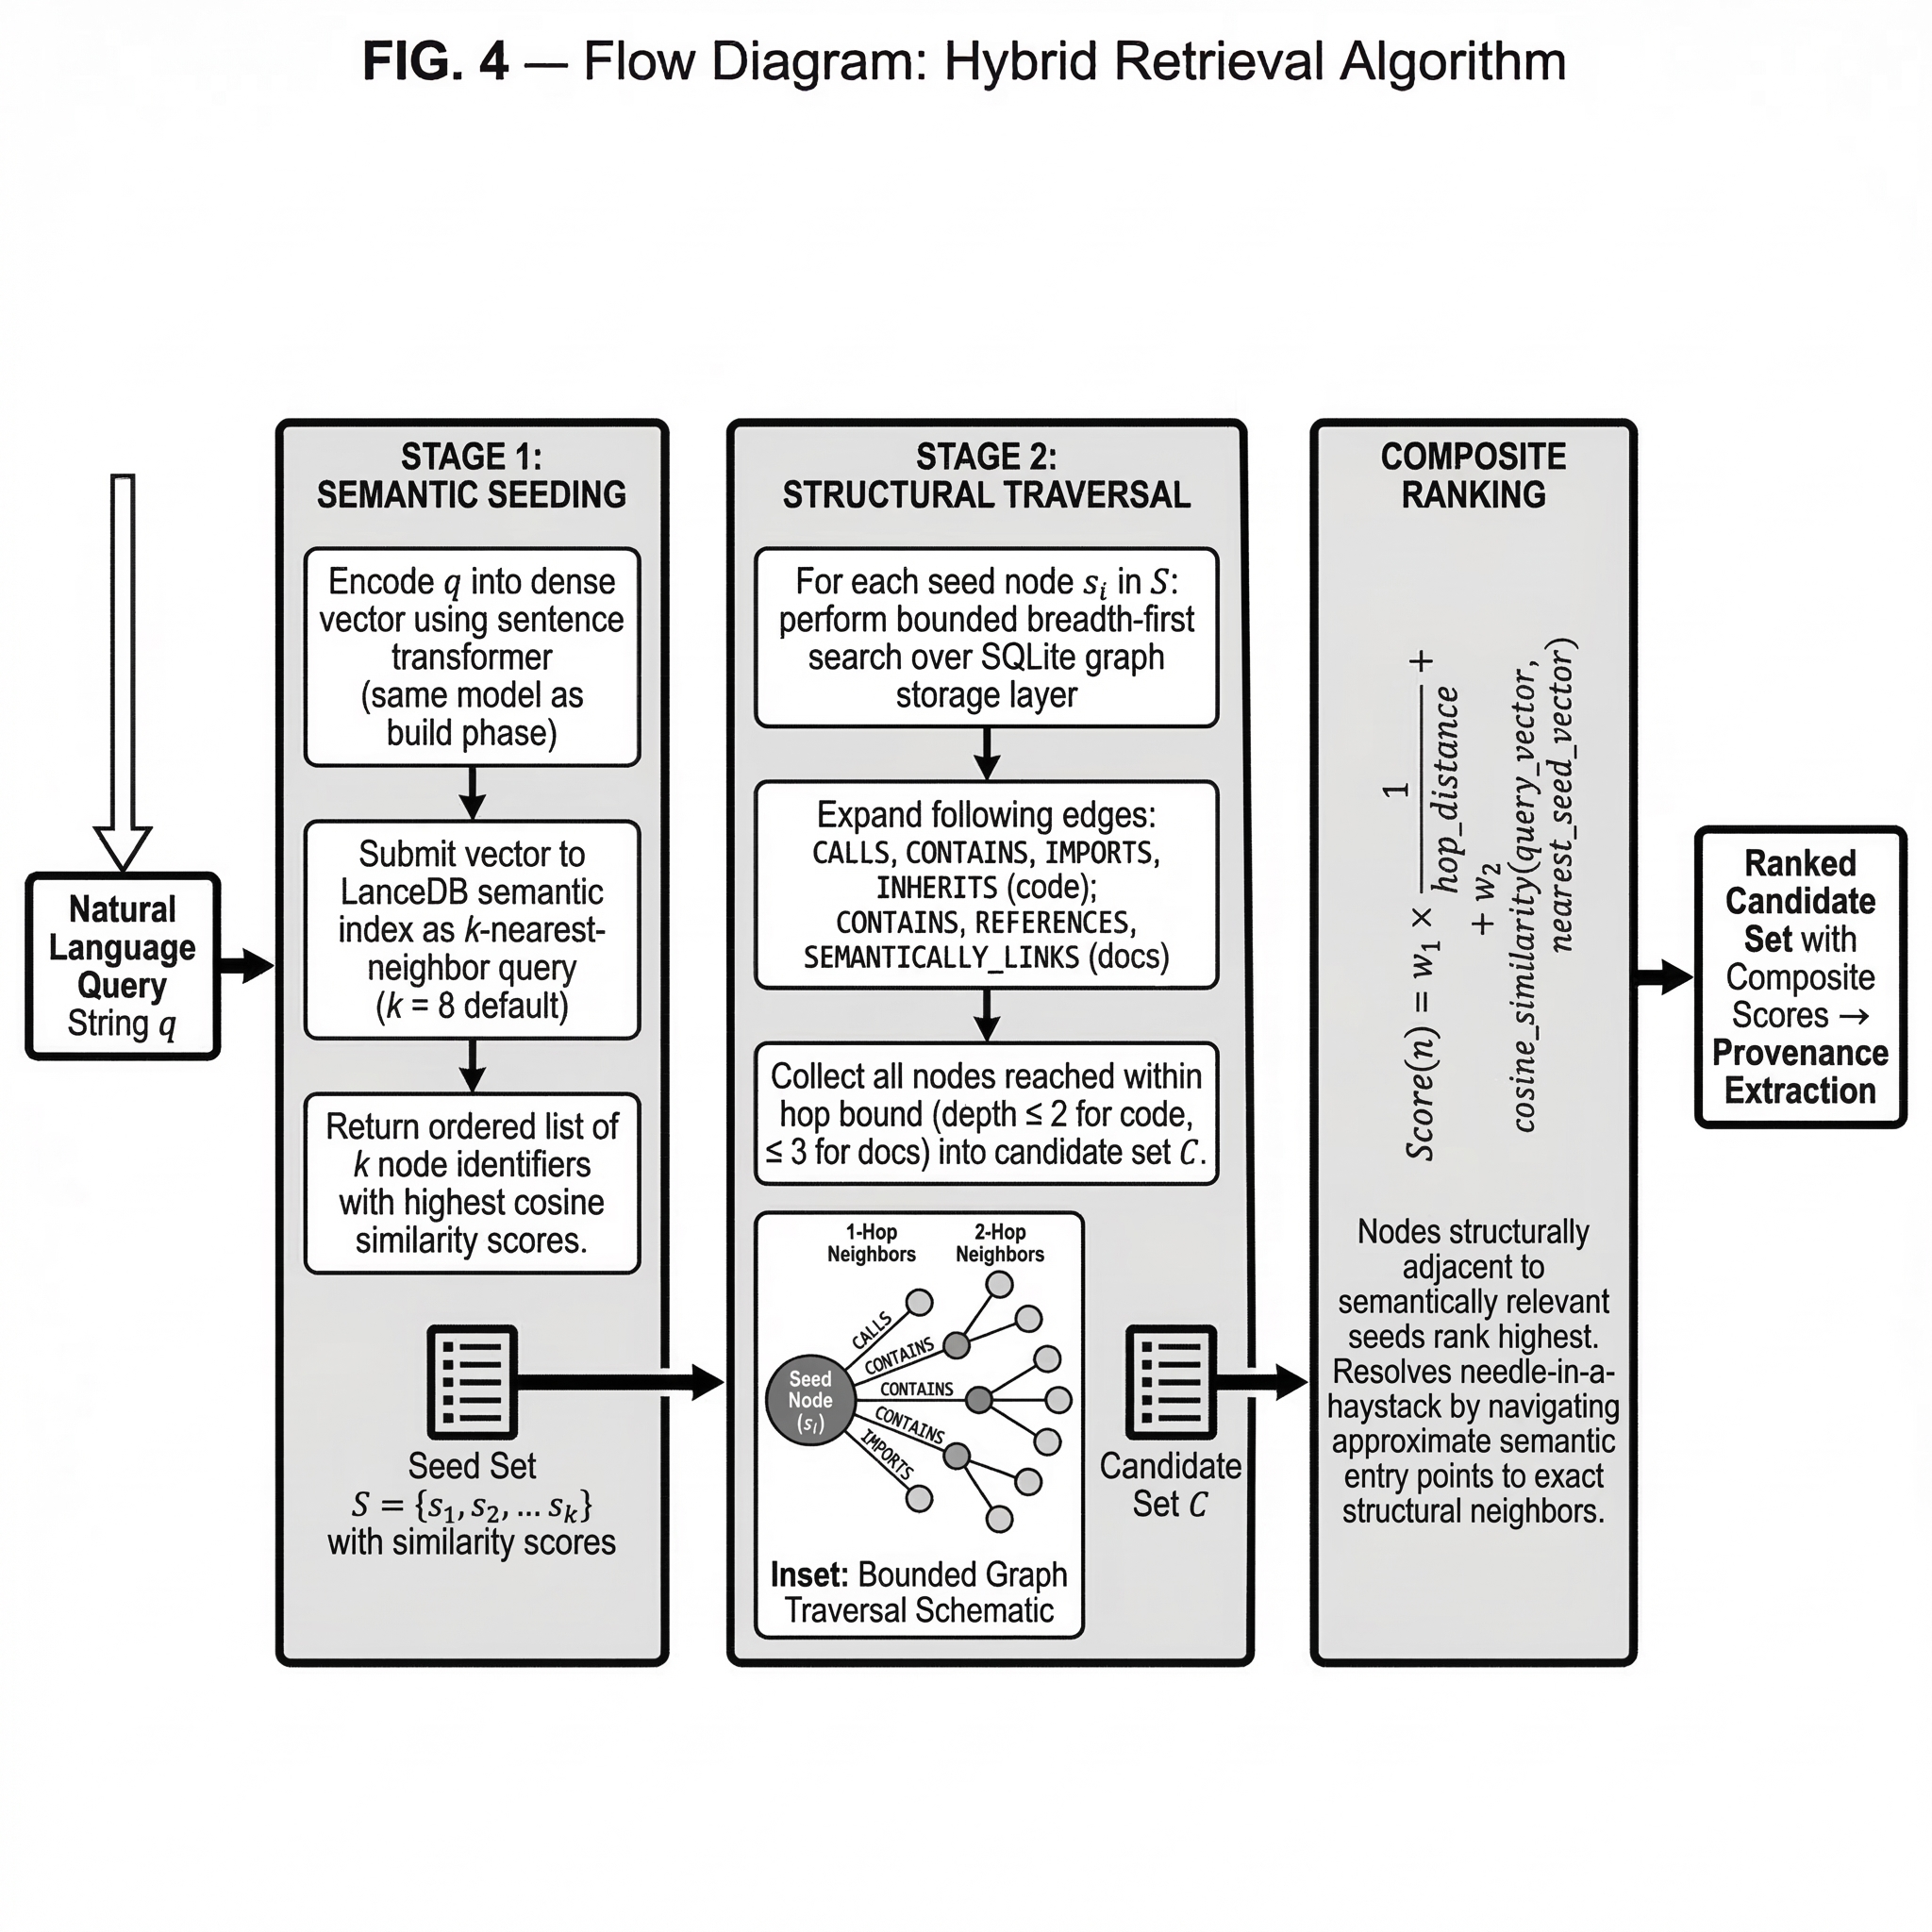
\includegraphics[width=0.95\textwidth]{fig4.png}
  \caption{The hybrid retrieval algorithm. Stage~1 (semantic seeding) encodes the
    query and retrieves $k$ nearest nodes from the vector index. Stage~2
    (structural traversal) performs bounded BFS from the seed nodes through the
    compiled graph. The composite ranking function ranks reached nodes by hop
    distance and seed similarity.}
  \label{fig:4}
\end{figure}

\subsubsection{IV.A\quad Stage~1: Semantic Seeding}

The semantic seeding stage accepts a natural language query string $q$. The
string is encoded into a dense vector using the same sentence transformer model
used during the build phase. The vector is submitted to the semantic index as a
$k$-nearest-neighbor query, returning a short ordered list of at most $k$ node
identifiers, in a preferred embodiment $k$ defaulting to eight, whose stored
vectors have the highest cosine similarity to the query vector. These $k$
identifiers constitute the seed set.

The semantic seeding stage has two properties that are critical to the correctness
of the overall retrieval:

\textbf{First,} it is not the final arbitrator of relevance. Its role is to
identify a small set of entry points into the compiled graph that are
semantically related to the query. The seed nodes are expected to be
approximately correct starting points, not necessarily the exact answer nodes.

\textbf{Second,} it is fast. A $k$-nearest-neighbor query over a LanceDB index of
tens of thousands of vectors requires milliseconds on commodity hardware. This
speed is possible because the embedding was computed and stored during the build
phase and need not be recomputed.

\subsubsection{IV.B\quad Stage~2: Structural Traversal}

The structural traversal stage accepts the seed set and the compiled graph.
Starting from each seed node, the stage performs a bounded breadth-first search
over the graph storage layer. The search follows directed edges whose relation
types are included in a configurable expansion set. For code knowledge graphs,
the default expansion set includes \texttt{CALLS}, \texttt{CONTAINS},
\texttt{IMPORTS}, and \texttt{INHERITS} edges. For documentation knowledge
graphs, it includes \texttt{CONTAINS}, \texttt{REFERENCES}, and
\texttt{SEMANTICALLY\_LINKS} edges.

The search is bounded by a configurable maximum hop depth, in a preferred
embodiment two hops for code graphs and three hops for documentation graphs. All
nodes reached within the hop bound are collected into a candidate set.

\subsubsection{IV.C\quad The Composite Ranking Function}

The candidate set is ranked by a composite key comprising two components: the hop
distance from the nearest seed node (lower is preferred), and the cosine
similarity to the query vector of the nearest seed node from which the candidate
was reached (higher is preferred). This ranking function ensures that nodes
directly connected in the compiled graph to semantically relevant entry points
are ranked higher than nodes that are semantically similar in isolation but have
no structural relationship to the query context.

This ranking function solves the needle-in-a-haystack problem as follows.
Consider a query for a specific function that is not mentioned by name in the
query string but is called by a function that is. The called function is a
semantic match for the query, and therefore appears in the seed set. The calling
function is reached in one hop from the seed node and ranked highly by the
composite function. A pure semantic retrieval system would not find this calling
function unless its canonical text happened to be semantically similar to the
query---which it may not be. The structural traversal finds it deterministically.

Referring to FIG.~\ref{fig:7}, the structural traversal addresses the
needle-in-a-haystack problem by using the compiled graph to navigate from
approximate semantic matches to exact structural neighbors, effectively converting
the global approximate search problem into a local exact navigation problem.

\begin{figure}[H]
  \centering
  
\includegraphics[width=0.92\textwidth]{fig7.png}
  \caption{The needle-in-a-haystack problem and its structural solution. Left:
    semantic search returns the most similar document, which is not the target.
    Right: structural traversal from a semantically adjacent seed node reaches
    the exact target via compiled graph edges.}
  \label{fig:7}
\end{figure}

% ---
\subsection{V.\quad Provenance-Grounded Synthesis and Hallucination Elimination}

Referring to FIG.~\ref{fig:6}, the present invention provides a synthesis
interface that ensures every fact available to a language model for synthesis is
directly traceable to a structurally verified source address.

\begin{figure}[H]
  \centering
  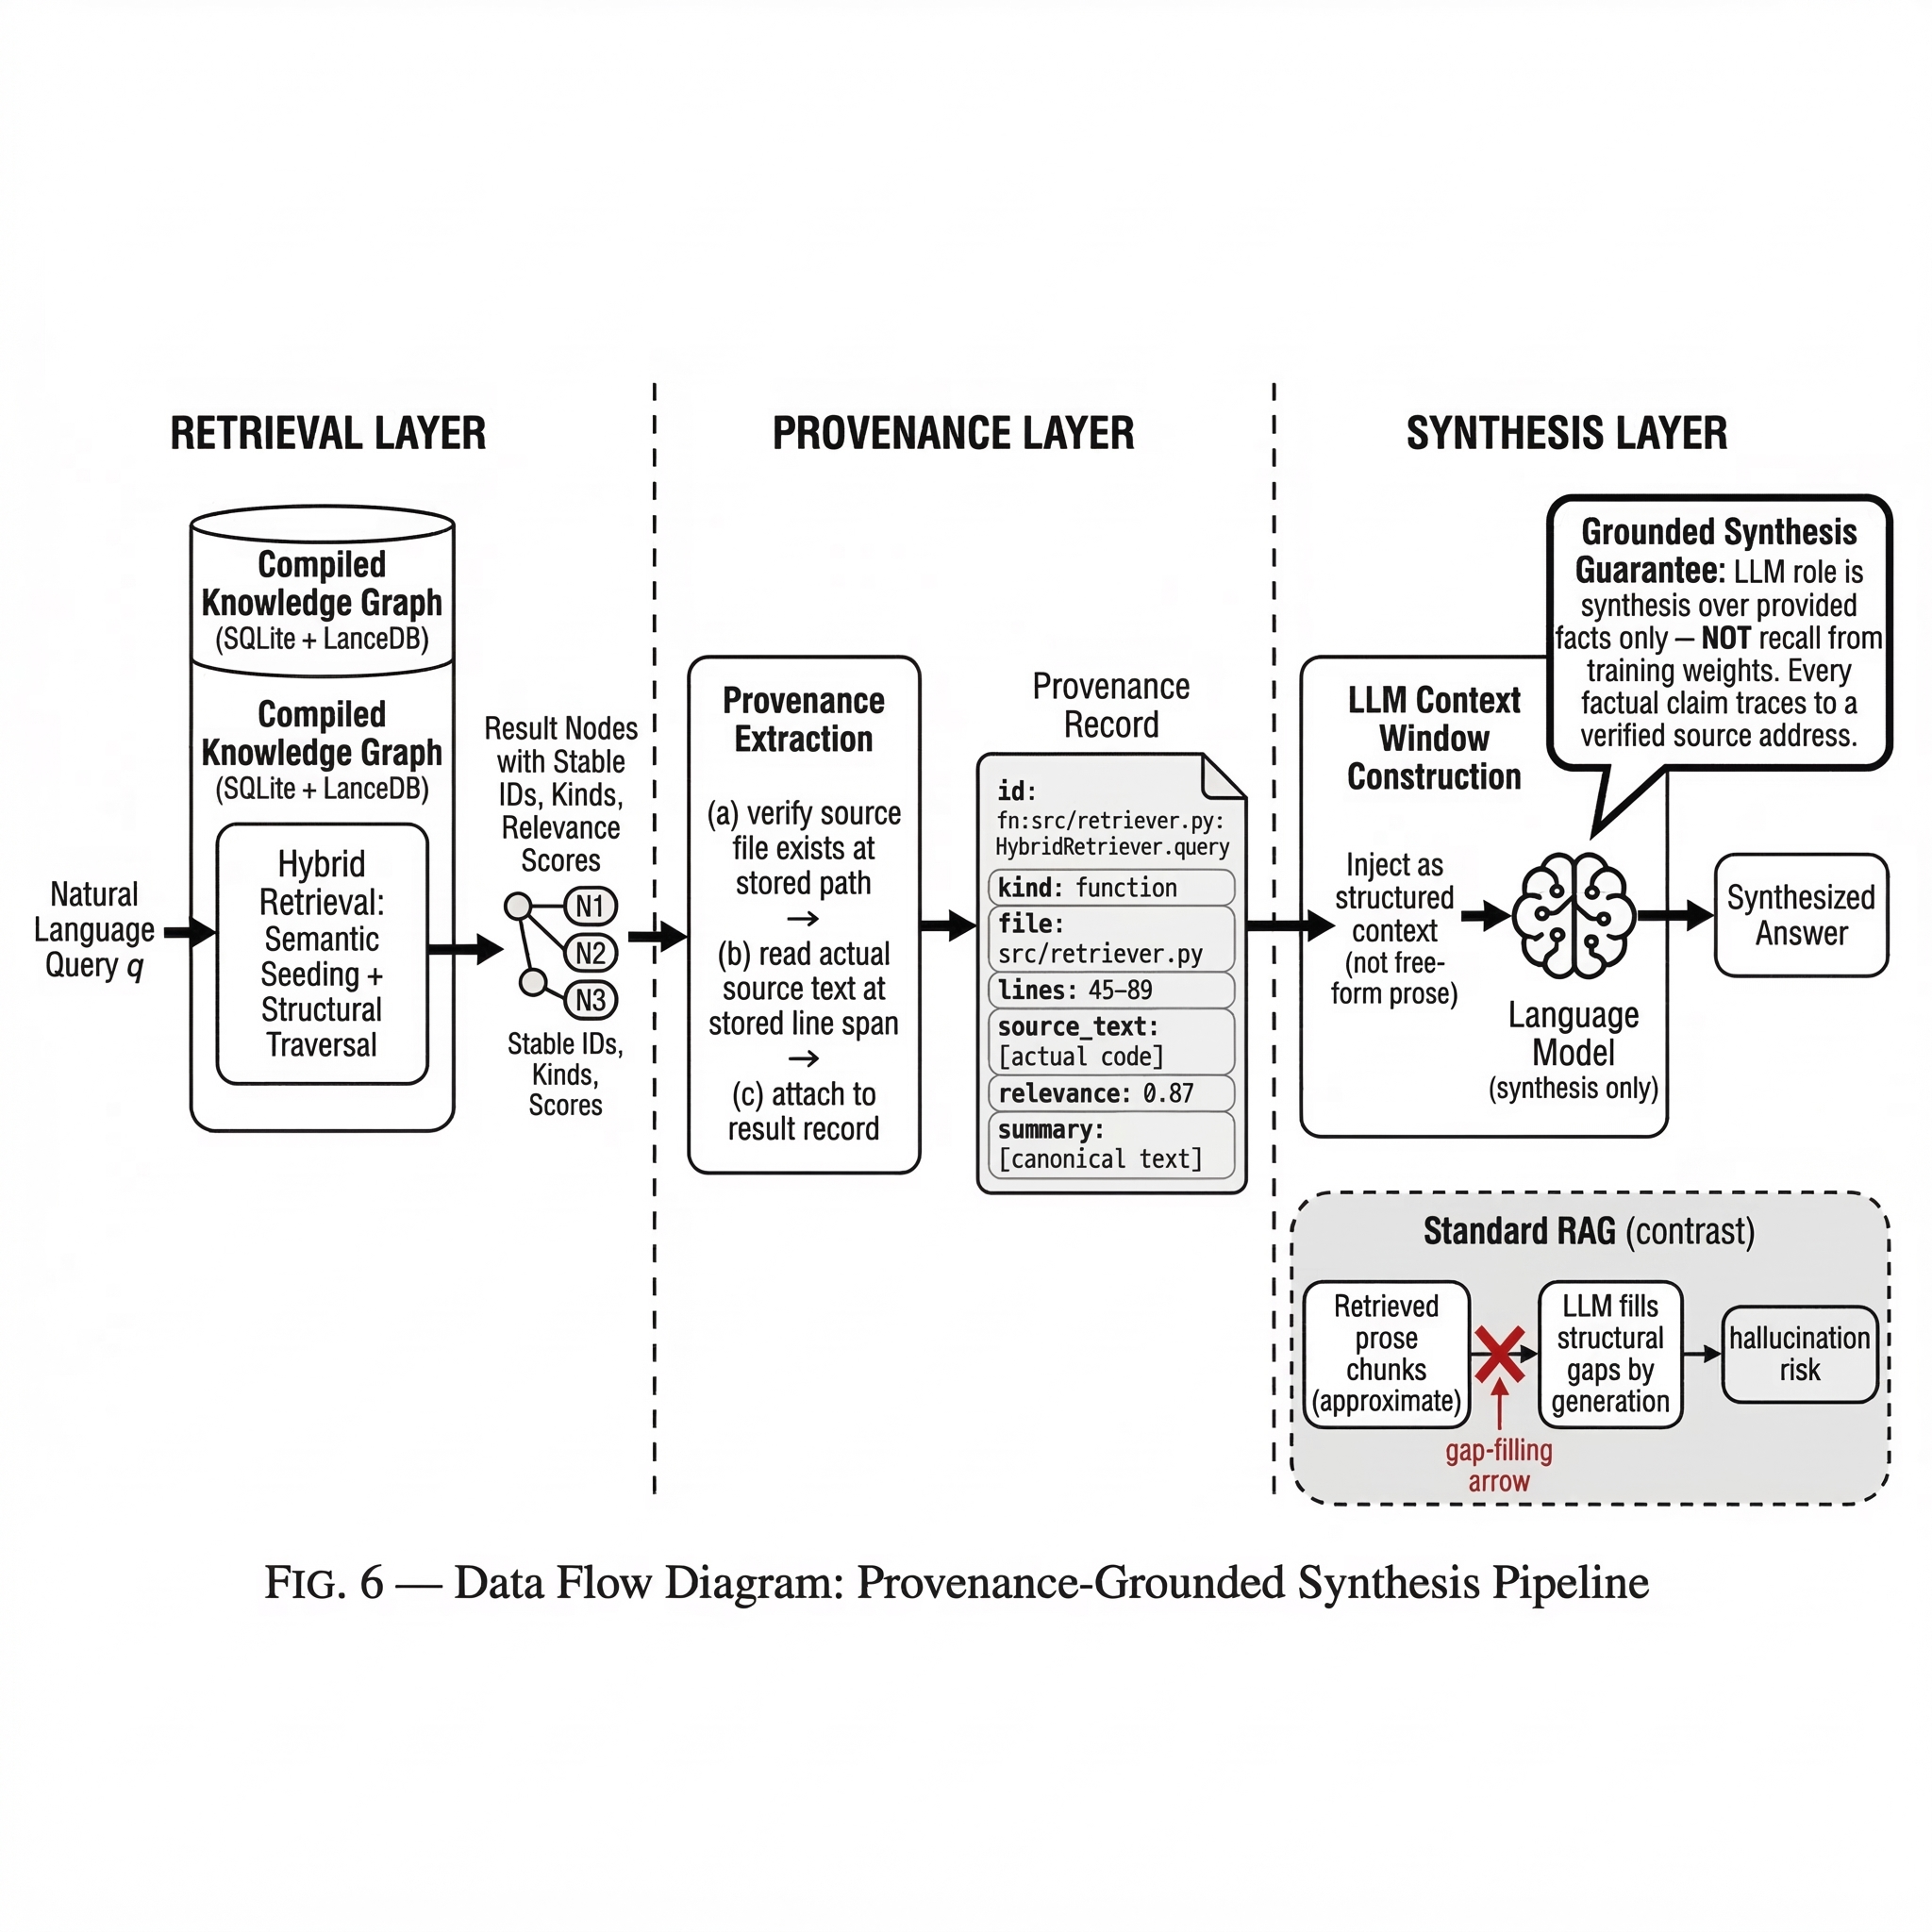
\includegraphics[width=0.92\textwidth]{fig6.png}
  \caption{The provenance-grounded synthesis pipeline. Provenance-tagged result
    records from the knowledge graph are injected into the LLM context window.
    The LLM synthesizes over verified facts, not trained weights.}
  \label{fig:6}
\end{figure}

\subsubsection{V.A\quad The Provenance Record}

After structural traversal and ranking, each result node in the candidate set is
enriched with a provenance record comprising:
\begin{enumerate}[label=(\alph*), leftmargin=2em]
  \item the stable node identifier, encoding kind, source file path, and
    qualified name as described in Section~III;
  \item the verified source file path;
  \item the start and end line numbers of the source text corresponding to the
    node, derived from the abstract syntax tree node spans or the document parser
    token offsets at build time;
  \item the actual source text read from the file at the stored line span,
    verified to exist at the time of retrieval;
  \item the relevance score from the composite ranking function; and
  \item a summary text string, which is the canonical text string constructed
    during Stage~3 of the build phase, not a generated summary.
\end{enumerate}

\subsubsection{V.B\quad The Grounded Synthesis Guarantee}

When provenance records are injected into an LLM context window and the LLM is
instructed to synthesize an answer from the provided records, a structural
guarantee holds: every statement in the synthesis is either directly present in
one of the injected provenance records or is a logical inference from statements
that are. No injected provenance record contains generated or approximated
content---each is actual source text at a verified address.

The LLM's role in this architecture is synthesis: connecting provided facts,
reasoning over their relationships, and formulating a response. The LLM is not
asked to recall facts from its training distribution, construct
plausible-sounding entities, or bridge gaps in provided context with guesses.
The set of facts available to the synthesis model is bounded and verified.

This grounded synthesis guarantee eliminates hallucination at the knowledge
layer: the system cannot produce factual claims about entities not present in the
compiled graph, because it does not retrieve entities not present in the compiled
graph, and because the synthesis model is constrained to the injected context.
The residual risk---reasoning errors over the provided facts---is distinct from
hallucination and is addressable by standard chain-of-thought verification and
re-querying techniques~\cite{wei2022chainofthought, yao2023react}.

\subsubsection{V.C\quad Comparison to Standard RAG}

In standard RAG~\cite{lewis2020rag}, retrieved chunks are segments of prose whose
content is approximately semantically related to the query. The synthesis model
may introduce hallucinated content by (a)~filling gaps between chunks with
generated text, (b)~misattributing the source of a statement, (c)~confusing
similar but distinct entities, or (d)~reasoning beyond the retrieved context
using training knowledge.

In the present invention, retrieved records are structurally defined entities
with verified source addresses. There are no gaps to fill---the structural graph
provides the connectivity. Misattribution is prevented by the stable node
identifier, which encodes the source address in a machine-readable, citable
format. Entity confusion is prevented by the node kind and identifier, which
uniquely identify each entity. Reasoning beyond context is addressed by providing
sufficient structural context through graph traversal to eliminate the need to
appeal to training knowledge.

% ---
\subsection{VI.\quad The Two-Pass AST Compiler for Python Source Code}

Referring to FIG.~\ref{fig:3}, the Python source code compiler is described in
detail as the primary preferred embodiment of the build-phase parser.

\begin{figure}[H]
  \centering
  
\includegraphics[width=0.95\textwidth]{fig3.png}
  \caption{The two-pass AST compiler for Python source code. Pass~1 (definition
    extraction) emits module, class, function, and method node records with
    \texttt{CONTAINS}, \texttt{IMPORTS}, and \texttt{INHERITS} edges. Pass~2
    (call-graph extraction) emits \texttt{CALLS} edges and resolves call-site
    stubs to first-party definitions via \texttt{RESOLVES\_TO} edges.}
  \label{fig:3}
\end{figure}

\subsubsection{VI.A\quad First Pass: Definition Extraction}

The first pass traverses the abstract syntax tree of every \texttt{.py} file in
the source repository. The traversal visits the following AST node types:
\texttt{Module} (one per file), \texttt{ClassDef}, \texttt{FunctionDef},
\texttt{AsyncFunctionDef}, and \texttt{Import} and \texttt{ImportFrom}
statements. For each visited node, the compiler emits:

A \emph{Module} node record with identifier \texttt{mo:relative\_path} and
metadata comprising the file's docstring, line count, and import list.

A \emph{Class} node record with identifier \texttt{cl:relative\_path:ClassName}
and metadata comprising the class's docstring, base class names, and decorator
names.

A \emph{Function or Method} node record with identifier
\texttt{fn:relative\_path:QualName} (where \texttt{QualName} is the
dot-qualified name within the module, e.g., \texttt{ClassName.method\_name} for
methods) and metadata comprising the function's docstring, parameter list, return
annotation, and decorator names. Coroutines receive a Boolean \texttt{is\_async}
field in their metadata.

A \emph{Symbol} node record for each module-level name assignment whose value is
a function reference, class reference, or constant that is referenced by other
nodes.

\texttt{CONTAINS} edges are emitted from each parent node to each child node
(module to class, class to method, module to top-level function).

\texttt{IMPORTS} edges are emitted from each module node to each imported module
or symbol, with the import path and alias stored as edge evidence.

\texttt{INHERITS} edges are emitted from each class node to each named base
class, with the base class expression stored as edge evidence.

\subsubsection{VI.B\quad Second Pass: Call Graph and Data-Flow Extraction}

The second pass traverses the abstract syntax tree a second time, this time
visiting \texttt{Call}, \texttt{Attribute}, and \texttt{Name} AST node types
within function and method bodies. For each \texttt{Call} node, the compiler
resolves the callee expression to a qualified name using a scope-tracking
resolver, emits a \texttt{CALLS} edge from the calling function or method node to
a call-site stub node, and records the call argument count and keyword argument
names as edge evidence.

A symbol resolution post-pass attempts to match each call-site stub node to a
first-party definition node by comparing the resolved qualified name to the set
of known function and method identifiers. Successful matches emit
\texttt{RESOLVES\_TO} edges from the stub node to the definition node. Unresolved
call-site stubs remain as nodes of kind \texttt{stub} and are available for query
but not traversal through \texttt{RESOLVES\_TO} edges.

\texttt{ATTR\_ACCESS} edges are emitted for each \texttt{Attribute} node whose
value is a \texttt{Name} node bound to a known object in scope.
\texttt{READS} and \texttt{WRITES} edges are emitted for \texttt{Name} nodes
appearing in \texttt{Load} and \texttt{Store} contexts, respectively, when the
name is bound to a known module-level or class-level symbol.

\subsubsection{VI.C\quad Determinism and Reproducibility}

The two-pass AST compiler is deterministic: for any given \texttt{.py} file and
Python version, it produces the same node records and edge records on every
invocation. Node identifiers are constructed from the same function of kind,
path, and qualified name on every invocation. This determinism enables the
stability guarantees described in Section~III.

% ---
\subsection{VII.\quad Multi-Domain Compiler Registry}

Referring to FIG.~\ref{fig:8}, the present invention provides a multi-domain
compiler registry that enables knowledge graphs compiled from heterogeneous
source domains to participate in a single retrieval interface.

\begin{figure}[H]
  \centering
  
\includegraphics[width=0.95\textwidth]{fig8.png}
  \caption{The multi-domain compiler registry. Domain-specific compilers for
    code, documentation, protein structure, legal statutes, diary corpora, and
    biochemical pathways all emit knowledge graphs conforming to a uniform node
    and edge interface, queryable through a single federated retrieval engine.}
  \label{fig:8}
\end{figure}

\subsubsection{VII.A\quad The Compiler Interface}

Each domain compiler is encapsulated in a compiler adapter class implementing a
uniform interface. The interface defines the following operations:

\texttt{is\_available} --- returns a Boolean indicating whether the
domain-specific parsing library required by this compiler is installed in the
current execution environment and whether a compiled graph exists at the
registered path.

\texttt{query(q, k)} --- accepts a query string and a result count, executes the
two-stage hybrid retrieval algorithm against this compiler's graph storage layer
and semantic index, and returns a ranked list of result records, each carrying a
stable node identifier, kind label, entity name, source file path, relevance
score, and summary text.

\texttt{pack(q, k, context)} --- extends \texttt{query} by reading the actual
source text at each result node's stored file path and line span and appending it
to the result record as a verbatim content field, producing provenance records
suitable for direct injection into an LLM context window.

\texttt{stats()} --- returns a dictionary containing at minimum the compiled
graph's node count and edge count, enabling monitoring, visualization, and
aggregate statistics across the registry.

\texttt{analyze()} --- returns a Markdown-formatted analytical report describing
the compiled graph's structural statistics, coverage metrics, and domain-specific
observations.

\texttt{snapshot(version, label)} --- captures the current compiled graph state,
persists it to durable storage keyed by the version-control tree hash of the
source corpus, and returns a serializable dictionary of graph metrics, enabling
differential queries between any two compiled states.

\texttt{\_graph\_stats()} --- a concrete method that invokes \texttt{stats()},
extracts the \texttt{node\_count} and \texttt{edge\_count} values, normalizes
them to integers, and returns them.

\subsubsection{VII.B\quad The Registry}

The registry is a persistent database, in a preferred embodiment
SQLite~\cite{sqlite}, storing one record per compiled knowledge graph instance.
Each record comprises: a universally unique identifier; a human-readable name;
a domain kind indicator from an enumerated set of supported domain kinds; the
absolute path to the source repository root; the path to the virtual Python
environment containing the domain compiler library; optional paths to the
compiled graph storage database and semantic index directory; a version string;
a list of tags; a dictionary of additional metadata; and creation and
modification timestamps.

The registry supports three grouping levels:

\textbf{Level~1, Individual Instances:} each compiled knowledge graph registered
independently with its own name and metadata.

\textbf{Level~2, Named Corpus Groups:} a named collection of individual instance
identifiers that can be queried as a unit through a single invocation.

\textbf{Level~3, Person Corpus Groups:} a named collection of individual instance
identifiers associated with a natural person, enriched with biographical metadata
including birth year, birth date, address, email, phone, and notes. Person corpus
groups are intended to aggregate all knowledge graphs relevant to a single
individual---code, documentation, diary, memory, correspondence---into a single
scoped query target.

\subsubsection{VII.C\quad Federated Retrieval over the Registry}

A federation orchestrator accepts a query string and iterates over all records in
the registry. For each record, the orchestrator calls \texttt{is\_available} on
the corresponding compiler adapter. For available adapters, the orchestrator
calls \texttt{query} and collects the returned result lists. After all available
adapters have been queried, the orchestrator merges the collected result lists and
sorts them by relevance score in descending order, producing a globally ranked
result list spanning all compiled knowledge graphs in the registry. The result
list carries per-result provenance including the source domain kind and the
registry instance name, enabling the recipient to identify not only the source
file and line but the knowledge graph and domain that produced each result.

% ---
\subsection{VIII.\quad The Hallucination-Elimination Theorem}

The present invention provides a structural argument---here stated informally as
a design theorem---explaining why the grounded synthesis architecture eliminates,
rather than merely reduces, hallucination at the knowledge layer.

\bigskip
\noindent\textbf{Theorem.}\quad Let $K$ be a compiled knowledge graph, let $R$ be
the result set produced by the hybrid retrieval algorithm for a query $q$ over
$K$, and let $C$ be the context window constructed from $R$ by the provenance
extraction stage. If a language model $M$ is constrained to synthesize its
response to $q$ using only $C$ as its knowledge source, then every factual claim
in $M$'s response is either:
\begin{enumerate}[label=(\alph*), leftmargin=2em]
  \item directly present as source text in a record in $R$; or
  \item a logical inference from facts that are directly present in $R$.
\end{enumerate}

No factual claim in $M$'s response can reference an entity, relationship, or
value that is not present in $K$, because:
\begin{enumerate}[label=(\roman*), leftmargin=2em]
  \item $R$ is a subset of $K$ by construction;
  \item $C$ is derived from $R$ by verbatim source text extraction, not
    generation;
  \item $M$ is constrained to $C$ for factual claims.
\end{enumerate}

The correctness of $K$ with respect to the source corpus follows from the
ontology-determinism principle: every node in $K$ corresponds to an entity in the
source corpus as defined by the formal specification; every edge corresponds to a
verified relationship. Therefore, every factual claim in $M$'s response is
traceable to a specific entity or relationship in the source corpus, at a
specific file path and line span.

This is not a property achievable by standard RAG~\cite{lewis2020rag}: in
standard RAG, $C$ contains approximate prose summaries, not verified source text;
retrieval is by global semantic proximity, not structural adjacency; and the
synthesis model is not structurally prevented from introducing content from its
training distribution.

% ---
\subsection{IX.\quad Graph Statistics and the Visible Corpus}

A consequence of the compiled-graph architecture that has no analogue in standard
RAG is that the structure of the knowledge base is directly observable. Because
the compiled knowledge graph is a relational database with typed nodes and edges,
structural statistics are computable by simple SQL aggregations:

\begin{lstlisting}[language=SQL, caption={Representative SQL statistics queries over the compiled knowledge graph.}]
-- Node distribution by kind
SELECT kind, COUNT(*) FROM nodes GROUP BY kind;

-- Edge distribution by relation type
SELECT relation, COUNT(*) FROM edges GROUP BY relation;

-- Module dependency depth (via IMPORTS traversal)
-- Call graph diameter (via RESOLVES_TO traversal)
\end{lstlisting}

These statistics are instantaneous and do not require re-parsing the source. They
expose properties of the compiled knowledge that are invisible to standard RAG
systems, which have no structural representation: the knowledge base is a flat
list of embedding vectors with no topology.

This observability enables diagnostic practices including: monitoring corpus
coverage over time via snapshot deltas; identifying under-indexed domains by low
node counts; detecting structural anomalies by unexpected edge distributions; and
visualizing the knowledge base topology through graph rendering tools.

% ---
\subsection{X.\quad Alternative Embodiments}

In alternative embodiments, the graph storage layer may use a graph database
management system such as Neo4j~\cite{neo4j}, ArangoDB, or TigerGraph in place
of SQLite, with the structural traversal stage adapted to use the graph
database's native traversal query language.

In alternative embodiments, the semantic indexing layer may use a vector database
other than LanceDB, including Chroma, Weaviate, Pinecone, Milvus, or
FAISS~\cite{johnson2021faiss}, with corresponding adaptations to the
$k$-nearest-neighbor query interface.

In alternative embodiments, the sentence transformer model used for canonical
text encoding may be replaced by any model producing fixed-dimensionality dense
vector representations, including domain-specific fine-tuned models,
sparse-dense hybrid models such as SPLADE~\cite{formal2021splade}, or
late-interaction models such as ColBERT~\cite{khattab2020colbert}, subject to
adaptation of the similarity computation in Stage~1.

In alternative embodiments, the bounded breadth-first structural traversal in
Stage~2 may be replaced by other graph traversal algorithms including depth-first
search, bidirectional BFS, personalized PageRank~\cite{page1999pagerank}, or
random walk with restart, with corresponding adaptation of the composite ranking
function.

In alternative embodiments, the stable node identifier format may encode
additional provenance fields including the content hash of the source file at
build time, enabling detection of source-level changes between compilation runs.

In alternative embodiments, the two-pass AST compiler for Python source code may
be extended with additional passes extracting type annotation edges, decorator
relationship edges, metaclass edges, and dataclass field edges.

In alternative embodiments, the formal specification used to derive the domain
ontology may itself be stored as a machine-readable artifact and versioned
alongside the source corpus, enabling automated detection of ontology changes
that require recompilation.

% -----------------------------------------------------------------------
\newpage
\section*{Claims}
% -----------------------------------------------------------------------

\noindent\textbf{Claim 1.}\quad
A computer-implemented system for compiling a structural knowledge graph from a
formally-structured source artifact, the system comprising:
\begin{itemize}[leftmargin=2.5em]
  \item one or more processors; and
  \item one or more non-transitory computer-readable media storing instructions
    that, when executed, cause the processors to perform:
    \begin{itemize}[leftmargin=2em]
      \item a \emph{parsing operation} that traverses the source artifact
        according to a domain ontology derived from the formal grammar or schema
        of the source artifact's domain, extracting typed entity records and
        directed relationship records without language model participation, each
        entity record comprising a stable identifier, a domain kind label, a
        canonical name, a source file path, a source line span, and a metadata
        dictionary;
      \item a \emph{graph storage operation} that persists the extracted entity
        records as node records and the extracted relationship records as edge
        records in a relational database;
      \item a \emph{canonical text construction operation} that constructs, for
        each node record, a canonical text string comprising the node's kind
        label, name, and available descriptive text;
      \item a \emph{semantic encoding operation} that encodes each canonical text
        string into a dense vector representation using a sentence transformer
        model and stores each vector in association with its node's stable
        identifier in a vector database;
      \item a \emph{semantic seeding operation} that, for a received query string,
        encodes the query string into a dense query vector using the same sentence
        transformer model and retrieves, from the vector database, an ordered list
        of at most $k$ node identifiers having the highest cosine similarity to
        the query vector;
      \item a \emph{structural traversal operation} that performs a bounded
        breadth-first search over the relational database starting from each node
        in the ordered list, following directed edges of configurable relation
        types up to a configurable maximum hop depth, and collecting all reached
        nodes into a candidate set; and
      \item a \emph{ranking operation} that ranks the candidate set by a composite
        key comprising the hop distance from the nearest seed node and the cosine
        similarity of that seed node to the query vector, and returns the ranked
        candidate set as the retrieval result.
    \end{itemize}
\end{itemize}

\bigskip
\noindent\textbf{Claim 2.}\quad
The system of claim~1, wherein the stable identifier for each entity record is
constructed deterministically as a concatenation of a kind prefix string, a
repository-relative source file path, and a qualified entity name or positional
index, such that any two executions of the parsing operation on the same source
artifact and the same ontology version produce identical stable identifiers for
the same entities.

\bigskip
\noindent\textbf{Claim 3.}\quad
The system of claim~1, wherein the parsing operation further performs a
\emph{provenance extraction operation} that, for each node in the ranked
candidate set, reads the actual source text at the node's stored source file path
and line span, verifies that the file exists at the stored path, and attaches the
read source text as a verbatim content field to the node's result record; whereby
every fact presented to a downstream language model for synthesis is directly
traceable to a verified source address and is actual source text rather than a
generated or approximated summary.

\bigskip
\noindent\textbf{Claim 4.}\quad
The system of claim~1, wherein the parsing operation for a Python source code
artifact comprises:
\begin{itemize}[leftmargin=2.5em]
  \item a \emph{first pass} that traverses the abstract syntax tree of each
    source file, extracts module, class, function, and method definition nodes,
    and emits \texttt{CONTAINS} edges from parent nodes to their contained
    children, \texttt{IMPORTS} edges from module nodes to referenced module
    names, and \texttt{INHERITS} edges from class nodes to their base class
    names; and
  \item a \emph{second pass} that traverses the abstract syntax tree a second
    time, extracts \texttt{Call}, \texttt{Attribute}, and \texttt{Name}
    expression nodes within function and method bodies, emits \texttt{CALLS}
    edges from calling function or method nodes to call-site stub nodes, and
    performs a post-pass symbol resolution step that emits \texttt{RESOLVES\_TO}
    edges from call-site stub nodes to first-party definition nodes whose
    qualified names match the resolved callee expression;
  \item whereby the compiled call graph is a deterministic theorem derived from
    the abstract syntax tree rather than a probabilistic inference.
\end{itemize}

\bigskip
\noindent\textbf{Claim 5.}\quad
The system of claim~1, wherein: the semantic encoding operation is performed
during a build phase that executes once per source corpus version; and the
semantic seeding operation, the structural traversal operation, and the ranking
operation are performed during a query phase that executes once per received query
string and performs no embedding model invocations; whereby the computational
cost of encoding is amortized over an unbounded number of subsequent queries and
each query executes in time bounded by the configured maximum hop depth
independent of corpus size.

\bigskip
\noindent\textbf{Claim 6.}\quad
The system of claim~1, further comprising:
\begin{itemize}[leftmargin=2.5em]
  \item a \emph{snapshot operation} that, when invoked with a version identifier
    and an optional label, reads the current node count and edge count from the
    relational database, captures domain-specific metrics from the compiled
    knowledge graph, constructs a snapshot record comprising the version
    identifier, an ISO~8601 UTC timestamp, the captured counts and metrics, and
    the optional label, and persists the snapshot record to a content-addressed
    file store keyed by the version identifier; and
  \item a \emph{differential query operation} that, given two version identifiers
    designating a first snapshot and a second snapshot, executes the retrieval
    algorithm against the knowledge graph state at each snapshot, computes the
    set difference of the top-$k$ result node identifier sets, and returns the
    node records present in the second result but absent from the first as
    representing knowledge that entered the compiled corpus between the two
    snapshots;
  \item whereby temporal changes in the compiled knowledge base are queryable as
    first-class operations.
\end{itemize}

\bigskip
\noindent\textbf{Claim 7.}\quad
The system of claim~1, further comprising:
\begin{itemize}[leftmargin=2.5em]
  \item a \emph{registry database} storing one record per compiled knowledge
    graph instance, each record comprising a unique identifier, a domain kind
    indicator, a repository path, and paths to the compiled graph storage
    database and vector database; and
  \item a \emph{federation orchestrator} configured to, for a received query
    string, iterate over records in the registry database, instantiate a compiler
    adapter for each record whose backing library is available and whose compiled
    graph files exist, invoke the retrieval algorithm of each instantiated
    adapter, collect all returned result records across all adapters, sort the
    collected records by relevance score in descending order, and return a
    globally ranked result list with per-result provenance identifying the source
    domain kind and registry instance name;
  \item whereby a single query string retrieves semantically and structurally
    relevant results from all compiled knowledge graphs in the registry without
    requiring the querier to know which knowledge graph contains the answer.
\end{itemize}

\bigskip
\noindent\textbf{Claim 8.}\quad
The system of claim~7, wherein the compiler adapter for each domain kind exposes
a uniform interface comprising: an availability check operation; the retrieval
operation; a snippet extraction operation that augments the retrieval result with
verbatim source text; a structural statistics operation returning at minimum node
count and edge count; an analysis operation returning a Markdown-formatted report;
and the snapshot operation; and wherein a stub adapter implementing the uniform
interface is instantiated for domain kinds whose backing libraries are not
installed, the stub adapter returning empty lists from retrieval and snippet
extraction, unavailability status from the statistics operation, and a minimal
dictionary from the snapshot operation; whereby new domain kinds can be registered
in the registry before their compilers are implemented without causing errors in
federation operations.

\bigskip
\noindent\textbf{Claim 9.}\quad
A computer-implemented \emph{method} for deterministic knowledge graph compilation
from a formally-structured source artifact, the method comprising:
\begin{itemize}[leftmargin=2.5em]
  \item receiving a source artifact whose structure is governed by a formal
    specification defining permissible entity types, relationship types, and
    grammar rules;
  \item deriving a compilation ontology from the formal specification, wherein the
    compilation ontology specifies a mapping from each entity type in the formal
    specification to a corresponding node kind in the knowledge graph, and a
    mapping from each relationship type or grammar rule in the formal
    specification to a corresponding directed edge type in the knowledge graph;
  \item traversing the source artifact according to the compilation ontology and
    emitting, for each entity encountered, a node record comprising a stable
    identifier constructed deterministically from the entity kind, source
    location, and qualified name, and for each relationship encountered, a
    directed edge record comprising the source node identifier, the edge type,
    and the destination node identifier;
  \item persisting the emitted node records and edge records to a relational
    database;
  \item constructing a canonical text representation for each persisted node and
    encoding the canonical text into a dense vector;
  \item storing each encoded vector in a vector database associated with the
    corresponding node's stable identifier; and
  \item responding to a query string by encoding the query string into a dense
    query vector, retrieving the $k$ nearest node identifiers from the vector
    database, expanding from those identifiers through the relational database by
    bounded breadth-first traversal of the stored edges, ranking the reached
    nodes by a composite function of structural distance and semantic similarity,
    and returning the ranked nodes with their stable identifiers and verified
    source text.
\end{itemize}

\bigskip
\noindent\textbf{Claim 10.}\quad
The method of claim~9, wherein the stable identifier for each node record is
constructed by concatenating a kind prefix that encodes the entity type, a
separator character, the repository-relative path of the source file containing
the entity, a separator character, and the dot-qualified name of the entity
within its file; and wherein the stable identifier uniquely identifies the entity
across all files in the source repository and is identical across any two
compilations of the same source artifact at the same corpus version.

\bigskip
\noindent\textbf{Claim 11.}\quad
The method of claim~9, further comprising:
\begin{itemize}[leftmargin=2.5em]
  \item after ranking, reading the actual source text at the source file path and
    line span recorded in each result node's node record;
  \item constructing a provenance record for each result node comprising the
    stable identifier, the source file path, the start line number, the end line
    number, and the verbatim source text read from the file; and
  \item presenting the collection of provenance records as a context window for
    injection into a language model prompt;
  \item wherein the language model, when instructed to synthesize a response using
    only the injected context window, is structurally constrained to produce
    factual claims that are either directly present as verbatim source text in
    the provenance records or are logical inferences from such text, thereby
    eliminating the possibility of the language model introducing factual claims
    about entities absent from the compiled knowledge graph.
\end{itemize}

\bigskip
\noindent\textbf{Claim 12.}\quad
The method of claim~9, wherein the source artifact is Python source code and the
compilation ontology is derived from the Python abstract syntax tree
specification, and wherein traversing the source artifact according to the
compilation ontology comprises:
\begin{itemize}[leftmargin=2.5em]
  \item performing a first traversal pass that visits \texttt{Module},
    \texttt{ClassDef}, \texttt{FunctionDef}, \texttt{AsyncFunctionDef}, and
    \texttt{Import} AST node types, emitting module node records, class node
    records, function and method node records, \texttt{CONTAINS} edges,
    \texttt{IMPORTS} edges, and \texttt{INHERITS} edges; and
  \item performing a second traversal pass that visits \texttt{Call},
    \texttt{Attribute}, and \texttt{Name} AST node types within function and
    method body subtrees, emitting \texttt{CALLS} edges to call-site stub nodes
    and performing symbol resolution to emit \texttt{RESOLVES\_TO} edges
    connecting call-site stubs to first-party definition nodes whose identifiers
    match the resolved callee qualified name.
\end{itemize}

\bigskip
\noindent\textbf{Claim 13.}\quad
The method of claim~9, wherein: the steps of traversing, persisting,
constructing, encoding, and storing are performed in a build phase that is
executed once per source corpus version and requires computational time
proportional to the number of nodes in the compiled knowledge graph; and the
steps of encoding a query string, retrieving nearest node identifiers, expanding
by traversal, ranking, and returning are performed in a query phase that is
executed once per query string and requires computational time bounded by a
product of the configured result count and the configured maximum traversal hop
depth, independent of the total number of nodes in the compiled knowledge graph.

\bigskip
\noindent\textbf{Claim 14.}\quad
The method of claim~9, further comprising: after the build phase is complete,
computing structural statistics by executing aggregate queries over the relational
database returning at minimum the total count of node records and the total count
of edge records partitioned by kind and relation type respectively; storing the
computed statistics as a snapshot record keyed by a content-addressable
identifier derived from the version-control state of the source artifact; and
upon request, computing a delta record by subtracting the node count and edge
count of a designated prior snapshot record from those of a designated current
snapshot record, and returning the delta record as a quantitative measure of the
structural change in the compiled knowledge graph between the two corpus versions.

\bigskip
\noindent\textbf{Claim 15.}\quad
A non-transitory computer-readable medium storing instructions that, when
executed by one or more processors, implement a knowledge compilation and
retrieval system comprising:
\begin{itemize}[leftmargin=2.5em]
  \item a \emph{compiler module} configured to, for a source artifact of a
    specified domain kind, apply a compilation ontology derived from the formal
    grammar or schema of that domain kind to extract a typed node set and a typed
    directed edge set from the source artifact without language model
    participation, construct a stable string identifier for each node encoding
    the node kind, source file path, and qualified entity name, and persist the
    node set and edge set to a structural graph database;
  \item a \emph{semantic index module} configured to construct a canonical text
    string for each persisted node and store a dense vector encoding of the
    canonical text in association with the node's stable identifier in a vector
    database;
  \item a \emph{retrieval module} configured to, for a received query string:
    encode the query string as a dense query vector; retrieve from the vector
    database a seed set of at most $k$ node identifiers having highest cosine
    similarity to the query vector; perform bounded breadth-first traversal of
    the structural graph database starting from each seed node, following
    directed edges of specified relation types up to a specified maximum hop
    depth; rank the collected traversal-reached nodes by a composite function of
    hop distance from the nearest seed and semantic similarity of that seed to
    the query; and return the ranked nodes;
  \item a \emph{provenance module} configured to, for each ranked node, read the
    verbatim source text at the node's stored file path and line span and attach
    it to the node's result record; and
  \item a \emph{synthesis interface module} configured to format the
    provenance-enriched result records as an injectable context window for a
    language model, wherein each record identifies its source by stable node
    identifier, file path, and line span.
\end{itemize}

\bigskip
\noindent\textbf{Claim 16.}\quad
The non-transitory computer-readable medium of claim~15, wherein the compiler
module is further configured to support a plurality of domain kinds by
maintaining a registry of domain-specific compilation ontologies, each ontology
specifying the node kinds, edge types, stable identifier construction function,
and traversal expansion edge set for its domain, such that adding support for a
new source domain requires specifying a new ontology without modifying the
retrieval module, the semantic index module, the provenance module, or the
synthesis interface module.

\bigskip
\noindent\textbf{Claim 17.}\quad
The non-transitory computer-readable medium of claim~15, wherein the retrieval
module is further configured to support federated retrieval over a plurality of
compiled knowledge graphs of heterogeneous domain kinds by:
\begin{itemize}[leftmargin=2.5em]
  \item maintaining a registry record for each compiled knowledge graph instance
    comprising the domain kind, the path to the structural graph database, and
    the path to the vector database;
  \item for a received query string, iterating over all registry records,
    instantiating a domain-specific compiler adapter for each record whose graph
    and index files are present, executing the retrieval algorithm against each
    adapter's graph and index, collecting all result records across all adapters,
    sorting the collected records by composite relevance score in descending
    order, and returning the globally sorted list with per-record source domain
    and instance name provenance.
\end{itemize}

% -----------------------------------------------------------------------
\newpage
\section*{Abstract of the Disclosure}
% -----------------------------------------------------------------------

A knowledge compilation system and method constructs structural knowledge graphs
from formally-structured source artifacts by deterministic parsing using
ontologies derived from the formal grammar or schema of each source domain,
without language model participation. Node identifiers encode kind, source path,
and qualified name to provide stable, citable addresses. A two-phase architecture
separates build-time compilation from query-time retrieval, amortizing embedding
cost over unbounded subsequent queries. Hybrid retrieval combines dense vector
semantic seeding with bounded breadth-first structural graph traversal from the
seed nodes, solving the needle-in-a-haystack problem by navigating compiled
structural relationships rather than relying solely on global semantic proximity.
Each retrieved node carries verbatim source text at a verified address,
structurally constraining a downstream language model to facts present in the
compiled graph and eliminating hallucination at the knowledge layer. A
multi-domain compiler registry enables federated retrieval across heterogeneous
compiled knowledge graphs through a uniform adapter interface.

% -----------------------------------------------------------------------
\newpage
\bibliographystyle{plain}
\bibliography{patent_1_knowledge_compiler}
% -----------------------------------------------------------------------

\end{document}
